\newcommand{\adwareTagResultsAucTable}{
    \begin{table}[H]
        \centering
        \begin{tabular}{|p{2,8cm}||P{2,4cm} P{2,4cm} P{2,4cm}|}
            \hline
            Adware Tag & ALOHA\newline (M/B only) & ALOHA & Proposed\newline Model \\
            \hline
            AUC-ROC & - & 0.969$\pm$0.004 & \textBF{0.976$\pm$0.000} \\
            \hline
        \end{tabular}
        \caption[Adware Tag prediction task AUC-ROC results]{AUC-ROC (Area Under Curve) of the different models for the \textbf{Adware Tag} prediction task. Results were aggregated over \textBF{2} training runs with different weight initializations and minibatch orderings. Best results are shown in \textbf{bold}.} \label{tab:adwareTag_auc}
    \end{table}
}

\newcommand{\adwareTagResultsAtFprTable}{
    \begin{center}
        \begin{longtable}[c]{|P{3,2cm}||P{1,8cm} P{1,8cm} P{1,8cm} P{1,8cm} P{1,8cm}|}
            \hline
            Adware Tag & \multicolumn{5}{c|}{{FPR}} \\
            & $10^{-5}$ & $10^{-4}$ & $10^{-3}$ & $10^{-2}$ & $10^{-1}$ \\
            \hline
            \endfirsthead

            \caption*{\raggedright ...continued from previous page} \\
            \hline
            Adware Tag & \multicolumn{5}{c|}{\textbf{FPR}} \\
            & $10^{-5}$ & $10^{-4}$ & $10^{-3}$ & $10^{-2}$ & $10^{-1}$ \\
            \hline
            \endhead

            \caption*{\raggedleft ...continued on next page} \\
            \endfoot

            \caption[Adware Tag prediction task results]{Mean and standard deviation results (TPR, Accuracy, Recall, Precision and F1-Score) of the different models for the \textbf{Adware Tag} prediction task at different \textbf{FPR}s (\textit{False Positive Rates}). Results were aggregated over \textBF{2} training runs with different weight initializations and minibatch orderings. Best results are shown in \textbf{bold}. Under \textbf{TPR} results are also presented the percentage reduction in mean detection error and in ROC curve standard deviation introduced by the \textit{Proposed Model} with respect to both \textit{ALOHA} model and \textit{Joint Embedding}.} \label{tab:adwareTag_results_at_fpr} \\
            \endlastfoot

            \multicolumn{6}{|c|}{\textbf{TPR}} \\
            \hline
            ALOHA (M/B only) & - & - & - & - & - \\
            ALOHA & \textBF{0.172$\pm$0.082} & 0.225$\pm$0.067 & 0.402$\pm$0.089 & 0.682$\pm$0.039 & 0.929$\pm$0.013 \\
            Proposed Model & 0.114$\pm$0.066 & \textBF{0.243$\pm$0.037} & \textBF{0.483$\pm$0.004} & \textBF{0.701$\pm$0.015} & \textBF{0.946$\pm$0.002} \\
            \hline
            Error Reduction wrt\newline ALOHA (M/B only) & - & - & - & - & - \\
            Error Reduction wrt\newline ALOHA & -7.0\% & 2.3\% & 13.5\% & 6.0\% & 23.9\% \\
            \hline
            Std Reduction wrt\newline ALOHA (M/B only) & - & - & - & - & - \\
            Std Reduction wrt\newline ALOHA & 19.5\% & 44.8\% & 95.5\% & 61.5\% & 84.6\% \\
            \hline
            \multicolumn{6}{|c|}{\textbf{Accuracy}} \\
            \hline
            ALOHA (M/B only) & - & - & - & - & - \\
            ALOHA & \textBF{0.952$\pm$0.005} & 0.955$\pm$0.004 & 0.965$\pm$0.005 & 0.972$\pm$0.002 & 0.902$\pm$0.001 \\
            Proposed Model & 0.949$\pm$0.004 & \textBF{0.956$\pm$0.002} & \textBF{0.969$\pm$0.000} & 0.973$\pm$0.001 & \textBF{0.903$\pm$0.000} \\
            \hline
            \multicolumn{6}{|c|}{\textbf{Recall}} \\
            \hline
            ALOHA (M/B only) & - & - & - & - & - \\
            ALOHA & \textBF{0.172$\pm$0.082} & 0.225$\pm$0.067 & 0.402$\pm$0.089 & 0.682$\pm$0.039 & 0.929$\pm$0.013 \\
            Proposed Model & 0.114$\pm$0.066 & \textBF{0.243$\pm$0.037} & \textBF{0.483$\pm$0.004} & \textBF{0.701$\pm$0.015} & \textBF{0.946$\pm$0.002} \\
            \hline
            \multicolumn{6}{|c|}{\textbf{Precision}} \\
            \hline
            ALOHA (M/B only) & - & - & - & - & - \\
            ALOHA & \textBF{0.999$\pm$0.001} & 0.992$\pm$0.002 & 0.959$\pm$0.009 & 0.806$\pm$0.009 & 0.362$\pm$0.003 \\
            Proposed Model & 0.998$\pm$0.001 & \textBF{0.993$\pm$0.001} & \textBF{0.967$\pm$0.000} & \textBF{0.811$\pm$0.003} & \textBF{0.366$\pm$0.001} \\
            \hline
            \multicolumn{6}{|c|}{\textbf{F1 Score}} \\
            \hline
            ALOHA (M/B only) & - & - & - & - & - \\
            ALOHA & \textBF{0.285$\pm$0.121} & 0.362$\pm$0.090 & 0.562$\pm$0.090 & 0.738$\pm$0.026 & 0.521$\pm$0.005 \\
            Proposed Model & 0.198$\pm$0.107 & \textBF{0.389$\pm$0.048} & \textBF{0.645$\pm$0.004} & \textBF{0.752$\pm$0.010} & \textBF{0.528$\pm$0.001} \\
            \hline
        \end{longtable}
    \end{center}
}

\newcommand{\adwareTagResultsSummaryTable}{
    \begin{table}[H]
        \centering
        \begin{tabular}{|P{3,2cm}||P{1,8cm} P{1,8cm} P{1,8cm} P{1,8cm} P{1,8cm}|}
            \hline
            \multicolumn{6}{|c|}{Adware Tag (at FPR $=1\%$)} \\
            \hline
            Model & TPR & Accuracy & Precision & Recall & F1 score \\
            \hline
            ALOHA (M/B only) & - & - & - & - & - \\
            ALOHA & 0.682$\pm$0.039 & 0.972$\pm$0.002 & 0.806$\pm$0.009 & 0.682$\pm$0.039 & 0.738$\pm$0.026 \\
            Proposed Model & \textBF{0.701$\pm$0.015} & 0.973$\pm$0.001 & \textBF{0.811$\pm$0.003} & \textBF{0.701$\pm$0.015} & \textBF{0.752$\pm$0.010} \\
            \hline
        \end{tabular}
        \caption[Summary of Adware Tag prediction task results]{Summary of the mean and standard deviation results of the different models for the \textbf{Adware Tag} prediction task at \textbf{FPR} $=1\%$. Results were aggregated over \textBF{2} training runs with different weight initializations and minibatch orderings. Best results are shown in \textbf{bold}.} \label{tab:adwareTag_result_summary}
    \end{table}
}

\newcommand{\adwareTagRocAlohaMB}{
    \begin{figure}[H]
        \vspace*{-0.5cm}
        \centering
        \includegraphics[width=0.6\textwidth]{./results/adware_tag_roc_alohaMB.png}
        \vspace*{-0.2cm}
        \caption[Adware Tag prediction task ALOHA (M/B only) ROC curve]{ROC curve and AUC statistics of \textBF{ALOHA (M/B only)} model for the \textbf{Adware Tag}. The line represents the \textit{mean} TPR at a given FPR, while the shaded region represents the \textit{standard deviation}. Statistics were computed over \textBF{2} training runs, each with random parameter initialization.}
        \label{fig:adwareTagRocAlohaMB}
    \end{figure}
}

\newcommand{\adwareTagRocAloha}{
    \begin{figure}[H]
        \vspace*{-0.5cm}
        \centering
        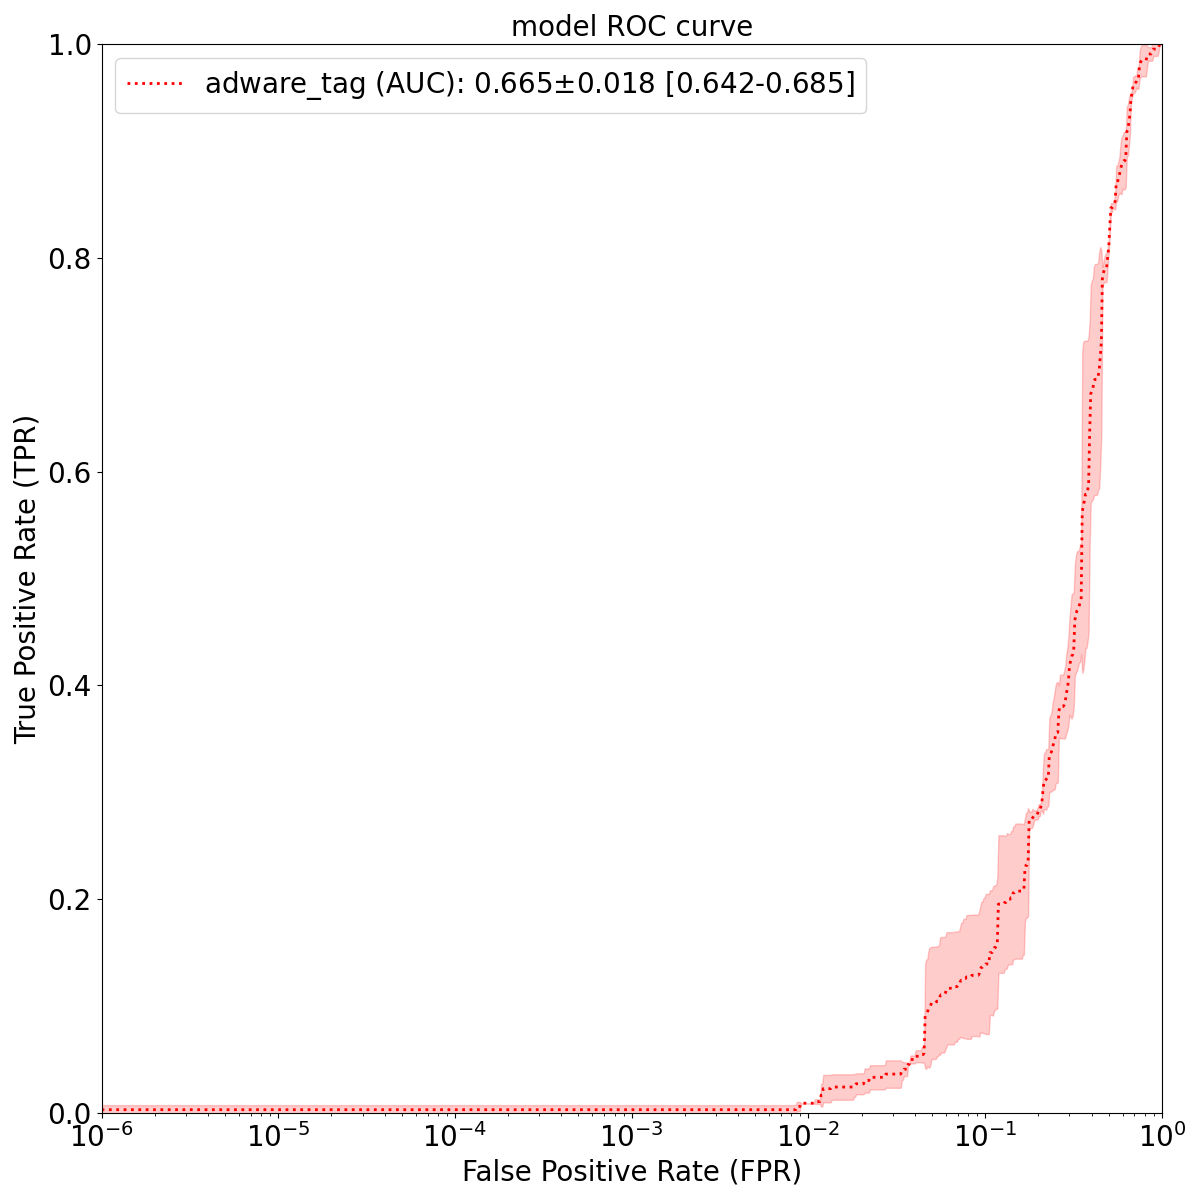
\includegraphics[width=0.6\textwidth]{./results/adware_tag_roc_aloha.png}
        \vspace*{-0.2cm}
        \caption[Adware Tag prediction task ALOHA ROC curve]{ROC curve and AUC statistics of \textBF{ALOHA} model for the \textbf{Adware Tag}. The line represents the \textit{mean} TPR at a given FPR, while the shaded region represents the \textit{standard deviation}. Statistics were computed over \textBF{2} training runs, each with random parameter initialization.}
        \label{fig:adwareTagRocAloha}
    \end{figure}
}

\newcommand{\adwareTagRocProposedMethod}{
    \begin{figure}[H]
        \vspace*{-0.5cm}
        \centering
        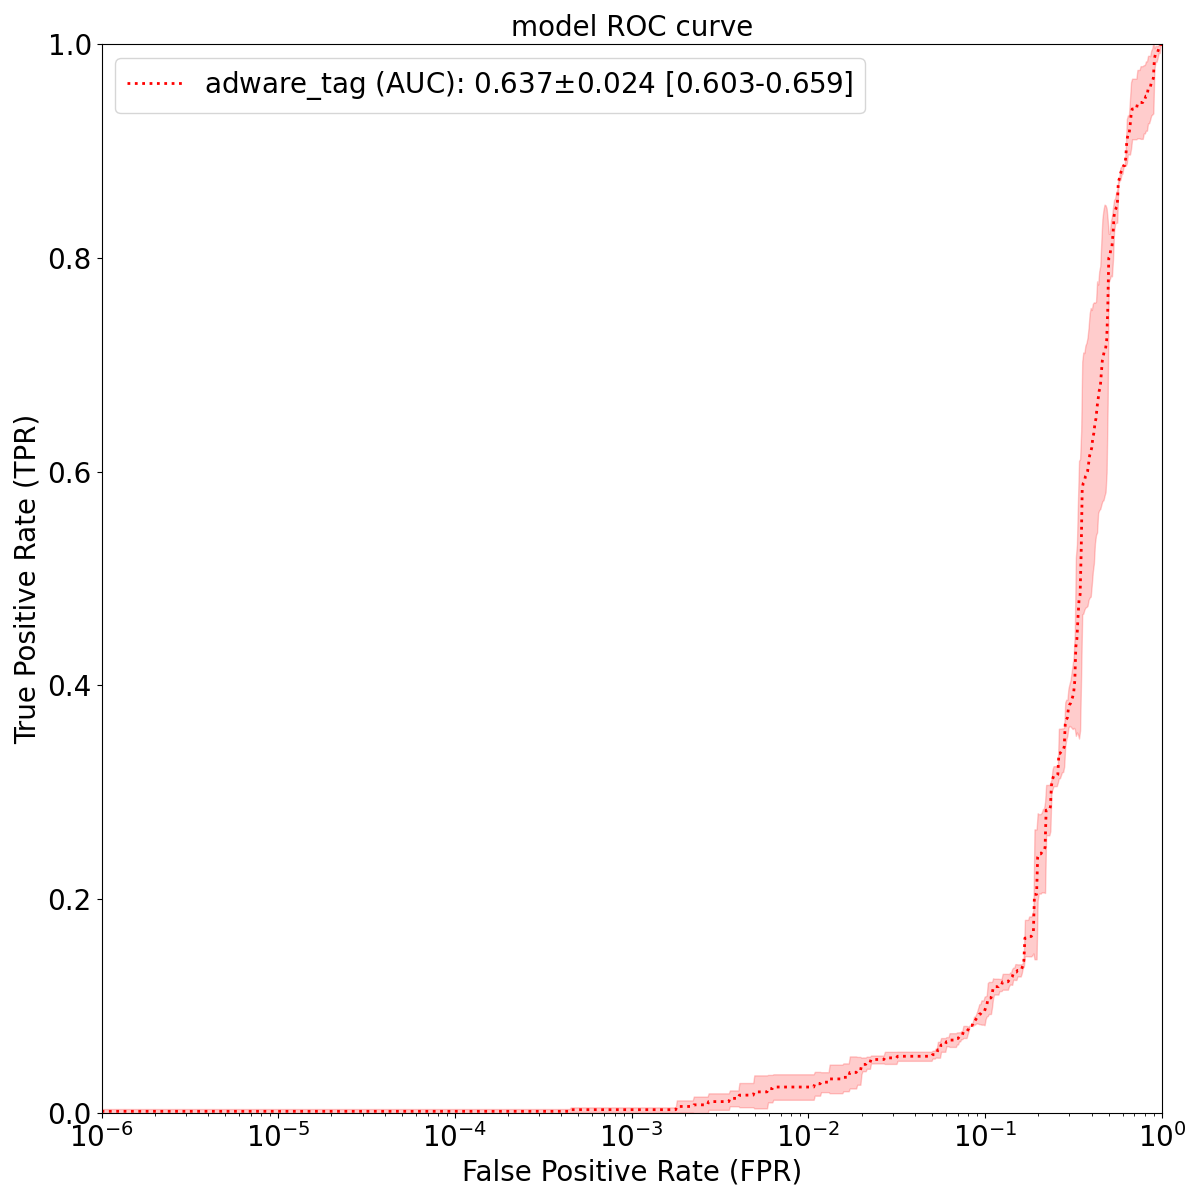
\includegraphics[width=0.6\textwidth]{./results/adware_tag_roc_proposedModel.png}
        \vspace*{-0.2cm}
        \caption[Adware Tag prediction task Proposed Model ROC curve]{ROC curve and AUC statistics of \textBF{Proposed Model} for the \textbf{Adware Tag}. The line represents the \textit{mean} TPR at a given FPR, while the shaded region represents the \textit{standard deviation}. Statistics were computed over \textBF{2} training runs, each with random parameter initialization.}
        \label{fig:adwareTagRocProposedModel}
    \end{figure}
}
